\documentclass[10pt]{article}
\usepackage[margin=1in]{geometry}
\usepackage[T1]{fontenc}
\usepackage{lmodern}
\usepackage{microtype}
\setlength{\emergencystretch}{1.5em}
\usepackage{amsmath,amssymb,amsthm,mathtools}
\usepackage{booktabs,multirow,tabularx}
\usepackage{graphicx}
\usepackage{xcolor}
\usepackage[numbers,sort&compress]{natbib}
\usepackage[colorlinks=true,linkcolor=blue!50!black,citecolor=blue!50!black,urlcolor=blue!50!black]{hyperref}
\usepackage[capitalise]{cleveref}

\newtheorem{definition}{Definition}
\newtheorem{proposition}{Proposition}
\newtheorem{remark}{Remark}
\newcommand{\R}{\mathbb{R}}
\newcommand{\Beta}{\mathrm{Beta}}
\newcommand{\cand}{\mathcal{C}}
\newcommand{\M}{\mathcal{M}}
\DeclareMathOperator*{\median}{median}
\DeclareMathOperator{\range}{range}
\newcommand{\nFamilies}{21}
\newcommand{\nWholeFam}{7}
\newcommand{\nTraits}{26}
\newcommand{\nTrainPerFamily}{40}
\newcommand{\nTrainScenes}{840}
\newcommand{\nTestPerFamily}{25}
\newcommand{\nTestScenes}{525}
\newcommand{\nValPerFamily}{12}
\newcommand{\nRobustPerFamily}{12}
\newcommand{\accAll}{73.1}
\newcommand{\pqAll}{86.6}
\newcommand{\accLo}{70.3}
\newcommand{\accHi}{76.2}
\newcommand{\accSingle}{86.0}
\newcommand{\accArranged}{34.0}
\newcommand{\accWhole}{92.0}
\newcommand{\pqArranged}{68.7}
\newcommand{\unitRecall}{62.2}
\newcommand{\aucAll}{0.802}
\newcommand{\fpLatent}{0.24}
\newcommand{\fpLogistic}{4.42}
\newcommand{\splitWholeLatent}{8.0}
\newcommand{\splitWholeLogistic}{88.6}
\newcommand{\accLogistic}{8.8}
\newcommand{\pqLogistic}{41.0}
\newcommand{\accEdge}{2.7}
\newcommand{\accNever}{33.5}
\newcommand{\pqNever}{58.1}
\newcommand{\accDefault}{50.7}
\newcommand{\accRelOn}{68.2}
\newcommand{\accNoAbst}{57.5}
\newcommand{\accCutsOnlySingle}{85.0}
\newcommand{\arrCutsOnly}{13.3}
\newcommand{\accRegionsOnlySingle}{13.5}
\newcommand{\arrRegionsOnly}{22.7}
\newcommand{\arrCarriedSeven}{17.3}
\newcommand{\curveOne}{49.9}
\newcommand{\curveForty}{73.1}
\newcommand{\lofoMean}{43.0}
\newcommand{\lofoMeanLogistic}{9.0}
\newcommand{\lofoSingle}{52.5}
\newcommand{\lofoArranged}{9.3}
\newcommand{\lofoWhole}{61.1}
\newcommand{\trSA}{5.3}
\newcommand{\trAS}{19.5}
\newcommand{\trSW}{75.4}
\newcommand{\trAW}{41.1}
\newcommand{\fsZero}{34.0}
\newcommand{\fsTen}{48.5}
\newcommand{\fsZeroSingle}{52.5}
\newcommand{\fsTenSingle}{66.8}
\newcommand{\fsZeroArranged}{9.3}
\newcommand{\fsTenArranged}{24.0}
\newcommand{\robRotNinety}{67.1}
\newcommand{\robRotOneEighty}{49.6}
\newcommand{\robScale}{59.5}
\newcommand{\robRecolour}{73.0}
\newcommand{\robDark}{73.0}
\newcommand{\robNoise}{44.4}
\newcommand{\robNoiseLogistic}{45.6}
\newcommand{\eceChosen}{0.467}
\newcommand{\eceOriginal}{0.025}
\newcommand{\baseRate}{3.3}
\newcommand{\oodRatio}{3.1}
\newcommand{\unitsFound}{62.2}
\newcommand{\arrMissed}{352}
\newcommand{\arrUnits}{787}
\newcommand{\missNoCand}{22.4}
\newcommand{\missNotCalled}{75.6}
\newcommand{\missBadly}{2.0}
\newcommand{\relTop}{edge\_lo, edge\_med, edge\_strong, edge\_hi}
\newcommand{\curveOneSingle}{50.7}
\newcommand{\curveFortySingle}{86.0}
\newcommand{\curveOneArranged}{15.6}
\newcommand{\curveFortyArranged}{34.0}
\newcommand{\curveOneWhole}{78.5}
\newcommand{\curveFortyWhole}{92.0}
\newcommand{\fsOne}{34.3}
\newcommand{\fsTwo}{34.6}
\newcommand{\fsFive}{41.1}
\newcommand{\secPerScene}{0.3}
\newcommand{\candPerScene}{170}
\newcommand{\missNoCandShelf}{55}
\newcommand{\missNoCandCabinet}{18}
\newcommand{\maxBooks}{29}
\newcommand{\nEquivAgree}{63}
\newcommand{\nEquivTotal}{63}
\newcommand{\chosenW}{0.005}
\newcommand{\chosenK}{4}
\newcommand{\chosenTheta}{0.5}
\newcommand{\nEntries}{103{,}975}
\newcommand{\nPositives}{951}
\newcommand{\valAcc}{77.8}
\newcommand{\valAccRel}{73.4}
\newcommand{\nValConfigs}{470}
\newcommand{\ablationText}{Every trait group contributes: removing the signal traits costs most (exact 60.2\% against 73.1\%), and no group alone comes close (the best, shape, reaches 44.6\%). The neighbourhood size matters most among the settings: at $k=96$ accuracy falls to 19.2\% with 3.16 false segments per scene, because with carried-whole entries counting almost nothing a large neighbourhood nearly always contains some part that came away. Raising the carried-whole weight trades recall for caution: at $w_0=1$ false segments fall to 0.11 per scene but unit recall falls to 28.8\% and accuracy to 60.6\%.}

\makeatletter
\newcommand{\tabinput}[1]{\@@input #1 }   % \input cannot open a file inside a tabular; the primitive can
\makeatother

\title{What Comes Apart: Observational Object Identity\\ and a Behavioural Latent Memory for Predicting Separable Parts}
\author{Anonymous author(s)}
\date{}

\begin{document}
\maketitle

\begin{abstract}
We study a definition of an object that is fixed entirely by observation: an object is a maximal set of sensed surface patches held together by contacts that have never been observed to open. Under this definition nothing is an object in advance; a scene begins as one object and divides only when something is seen to move apart, and the division is permanent. The definition is exact but silent about things that have not yet moved. We add a second layer that may speak about them without ever changing identity: a memory of observations in which every entry is a candidate part described by \emph{physical traits} (size, shape, how it touches the rest, how the sensed signal changes across that contact, where it sits) together with its \emph{recorded behaviour}---whether that part was seen to come away or was carried whole. A part of an unmoved object is predicted to separate when its nearest stored neighbours in the standardised trait space carry enough kernel-weighted evidence that they did; otherwise the memory says the part stays joined, or abstains. All labels come from the definition; nothing in the system names a kind of object. In a controlled 2-D world with patch-level sensing and a scripted hand, we evaluate on \nFamilies{} families---single objects with caps and lids, everyday arrangements (books in a shelf, things on a table, drawers in a cabinet, fruit in a bowl, pencils in a cup, a stack of books) and things that never come apart (hammers, chairs, mugs, lamps). Trained on \nTrainScenes{} handled scenes, the memory reproduces the exact ground-truth partition of \accAll\% of unseen still scenes (panoptic quality \pqAll\%), against \accLogistic\% for logistic regression on the same traits and \accEdge\% for a boundary-contrast rule. We report learning curves, leave-one-family-out transfer, few-shot teaching, ablations, robustness to rotation, scale and colour changes, calibration and abstention, and we state the limits of a synthetic study plainly.
\end{abstract}

\section{Introduction}

What is an object? Datasets for detection and segmentation answer by annotation: an object is whatever an annotator outlined \citep{lin2014coco,kirillov2023sam}. Developmental psychology offers a physical answer instead: infants treat as one object what moves as one connected, bounded body \citep{spelke1990principles}, an idea that goes back to the Gestalt principle of common fate \citep{wertheimer1923}. Computer vision and robotics have used motion and interaction to discover objects for this reason \citep{metta2003better,katz2008manipulating,vanhoof2014probabilistic,bohg2017interactive,pathak2017watching,pathak2018interaction,yang2021motiongroup,bao2022discovering}.

We take the physical answer to its end point and make it a definition. An object is a maximal set of sensed patches held together by interfaces that have never been observed to open (\cref{sec:definition}). The definition needs no categories, no appearance model and no training; it says exactly when identity changes (only when a contact is seen to open), and it satisfies strong invariants: separation is permanent, identity survives motion, articulation, contact and occlusion. Its price is equally clear: before anything moves, a bookshelf with its books is one object, and so is a table with the cups on it.

The question we ask is how a system holding \emph{only} this definition can come to say something useful about objects that have not moved yet, without giving up any of the definition's guarantees. Our answer is a second, separate layer: a \emph{latent memory of observations}. Whenever the definition records an event---a part came away, or a piece was carried whole---the system stores the physical traits of the parts involved together with that recorded behaviour. A new, unmoved scene is read by placing its candidate parts in the same trait space and asking what their nearest stored neighbours did. The layer predicts but never decides: object identity is computed by the definition alone, from observations alone (\cref{prop:identity}).

\paragraph{Contributions.}
(i) A formal two-layer account of objects: an observational identity layer and a predictive layer whose hypotheses provably cannot alter identity (\cref{sec:definition,sec:memory}).
(ii) A signal-agnostic description of a candidate part of any shape by \nTraits{} physical traits, with candidate parts from straight cuts and from regions of the sensed signal, and stated invariances (\cref{sec:traits}).
(iii) A nonparametric memory with a kernel-weighted Beta posterior, a credible-bound decision rule and principled abstention, with properties proved (\cref{sec:memory}), and a learning rule that takes every label from the definition (\cref{sec:learning}).
(iv) An evaluation on \nFamilies{} families of objects and arrangements in a controlled world, with baselines, ablations, transfer, few-shot, robustness and calibration studies, and a check that the offline evaluation reproduces the live system exactly (\cref{sec:experiments,sec:results}). It includes two negative findings that shaped the final design: weighting traits by their separating power, our original design, lowered accuracy on validation scenes, and entries recording that a part was carried whole are nearly worthless as evidence against its coming apart.

\section{Related work}
\label{sec:related}

\paragraph{Objects from motion and interaction.}
Common fate \citep{wertheimer1923} and infants' object principles of cohesion and boundedness \citep{spelke1990principles} motivate grouping by joint motion. \citet{metta2003better} used a robot's own pokes to segment what moves; \citet{katz2008manipulating} recovered articulation by interaction; \citet{vanhoof2014probabilistic} chose informative pushes under a probabilistic segmentation model; \citet{bohg2017interactive} survey this interactive-perception line. With deep networks, \citet{pathak2017watching} used motion segments in video as free targets for a network that segments single frames; \citet{pathak2018interaction} trained instance segmentation from a robot's own grasps; \citet{yang2021motiongroup} group optical flow into objects without labels; \citet{bao2022discovering} show that a weak motion signal transfers to static instances of things that can move. Object-centric models learn slots from images or video \citep{locatello2020slot,kipf2022savi}. Our work shares the premise that motion reveals objects. It differs in that (a) identity is a \emph{definition} with proved invariants, not a learned segmentation, so the learned part can never overrule what was observed, and (b) the learned part is a memory of discrete, inspectable observations that predicts a \emph{behaviour} (coming apart) rather than a mask.

\paragraph{Objects in cognition.}
Object files keep an object's identity through change by spatiotemporal continuity rather than by appearance \citep{kahneman1992objectfiles}, which is close to how our definition carries identity through motion and occlusion. That what a thing \emph{affords}---here, whether it comes apart---is perceived directly from its form is Gibson's ecological view \citep{gibson1979ecological}; our memory makes that link learned and explicit. \citet{lake2017building} argue that machines should learn from few examples by building on structured knowledge of objects and physics; the few-shot behaviour of our memory is bounded in a precise way (\cref{prop:evidence}).

\paragraph{Parts and mobility.}
The minima rule places part boundaries at concavities \citep{hoffman1984parts}; recognition-by-components treats objects as arrangements of parts \citep{biederman1987rbc}. \citet{hu2017mobility} predict part mobility from a single static 3-D snapshot using a learned snapshot-to-unit distance, and \citet{mo2021where2act} learn where actions on articulated objects succeed. These are close in spirit---behaviour predicted from static form---but rely on segmented 3-D shapes or simulated interaction with labelled articulation; here parts are proposed from raw patches and every label comes from the observational definition.

\paragraph{Nearest neighbours, metric weighting and abstention.}
Our reader is a $k$-nearest-neighbour rule \citep{cover1967nn} with an adaptive kernel; $k$-NN regression is universally consistent when $k\to\infty$ and $k/n\to0$ \citep{stone1977consistent}, which our fixed $k$ does not satisfy (\cref{rem:consistency}). We also tried weighting traits by a per-coordinate Fisher criterion \citep{fisher1936lda}, a far simpler choice than learned metrics such as LMNN \citep{weinberger2009lmnn}; validation rejected it. The reject option goes back to \citet{chow1970reject}; selective prediction is studied by \citet{geifman2017selective}. We measure calibration with the expected calibration error \citep{guo2017calibration} and partitions with panoptic quality \citep{kirillov2019panoptic}.

\section{Objects by observation}
\label{sec:definition}

Time is discrete, $t\in\{1,\dots,T\}$. $P_t$ is the set of patches known at $t$ ($P_t\subseteq P_{t+1}$; correspondence over time is given), $V_t\subseteq P_t$ the patches observed at $t$, $x_a(t)\in\R^2$ the position and $\sigma_a(t)\in\R^c$ the signal sensed by patch $a$. With a contact distance $\varepsilon$ and a persistence $k$, each pair $a,b\in P_t$ is in exactly one state:
\emph{adjacent}, $(a,b)\in A_t$, if $a,b\in V_t$ and $\lVert x_a(t)-x_b(t)\rVert\le\varepsilon$;
\emph{apart}, $(a,b)\in N_t$, if $a,b\in V_t$ and the distance has exceeded $\varepsilon$ for $k$ consecutive observations;
\emph{undetermined} otherwise. Let $\tau(a,b)=\min\{s:(a,b)\in A_s\cup N_s\}$ be the pair's first determination.

\begin{definition}[Interfaces and objects]\label{def:object}
A pair is a \emph{candidate interface} if it was adjacent when first determined, $\mathrm{Cand}(a,b)\Leftrightarrow(a,b)\in A_{\tau(a,b)}$. It is \emph{open} at $t$ if it has been apart since, $\mathrm{Open}_t(a,b)\Leftrightarrow\exists s\in[\tau(a,b),t]:(a,b)\in N_s$. Starting from $I_0=\emptyset$, at each $t$: remove every interface in $N_t$; consider the new candidates ($\tau=t$) in decreasing order of a preference $\pi$ and admit each unless it would join two patches that were in different objects at $t-1$. The objects $O_t$ are the connected components of $(P_t,I_t)$.
\end{definition}

Interfaces are never recreated, so separation is permanent; identity persists through motion, articulation (a chain of unopened interfaces suffices), contact formed later, and occlusion (an undetermined pair never opens). An object $U\in O_{t'}$ is \emph{divided} by $t>t'$ if its patches lie in more than one object of $O_t$. In this paper $\pi$ is a fixed colour-continuity score between neighbouring patches; it is used only to order the admission of new interfaces and is never learned.

\begin{proposition}[Identity does not depend on the memory]\label{prop:identity}
Let $O_t(\M)$ denote the objects computed while the predictive layer holds memory $\M$. For any memories $\M,\M'$ and the same observations, $O_t(\M)=O_t(\M')$ for all $t$.
\end{proposition}
\begin{proof}
By \cref{def:object}, $I_t$ is a function of $(A_s,N_s)_{s\le t}$, of $\pi$, and of $O_{t-1}$; $O_t$ is a function of $I_t$. $A_s,N_s$ depend only on positions and visibility; $\pi$ is fixed. By induction on $t$ ($O_0=\emptyset$), $O_t$ is a function of observations only. The predictive layer reads $O_t$ but writes nothing that enters this recursion.
\end{proof}

\section{Candidate parts and their physical traits}
\label{sec:traits}

Fix an object $O\in O_t$ with $n=|O|$ visible patches on a lattice of spacing $s$. Its \emph{contacts} are $E_O=\{(a,b)\in O^2:\lVert x_a-x_b\rVert\le1.05\,s\}$ (4-neighbours). The \emph{normalised change} across a contact is
\begin{equation}
\delta_{ab}=\frac{\lVert\sigma_a-\sigma_b\rVert}{m_O+\nu},\qquad m_O=\median_{(a,b)\in E_O}\lVert\sigma_a-\sigma_b\rVert,\qquad \nu=3,
\end{equation}
i.e.\ in units of the object's own typical neighbour difference; $\nu$ is a noise floor in signal units.

\paragraph{Candidates.} A candidate part is a set $C\subset O$, $3\le|C|$. Two generators propose them.
\emph{Cuts:} for directions $\theta\in\Theta=\{0^\circ,45^\circ,90^\circ,135^\circ\}$ and every lattice offset $c$, the smaller side of $\{a:\langle x_a,u_\theta\rangle<c\}$.
\emph{Regions:} for thresholds $\lambda\in\Lambda=\{1.5,3,6,12\}$, the connected components of $(O,\{e\in E_O:\delta_e\le\lambda\})$ with at most $0.8\,n$ patches (the 40 largest per $\lambda$), each with its holes filled on the lattice (a label on a book belongs to the book). $\cand(O)$ is the union without duplicates. Cuts express parts on one side of a line (a cap, a lid); regions express parts bounded on several sides by the rest (a book among books, a drawer in a cabinet, one cup among several on a table).

\paragraph{Traits.} Let $R=O\setminus C$, let $E_\times=\{(a,b)\in E_O:a\in C,b\in R\}$ be the contacts between part and rest, $\partial_RC$ the patches of $C$ on such a contact, $\partial C=\partial_RC\cup\{a\in C:a\text{ has an empty 4-neighbour cell}\}$ the part's rim, and $R_\partial$ the patches of $R$ on such a contact. For a point set $Q$ write $\bar x(Q)$ for its centroid, $\lambda_1(Q)\ge\lambda_2(Q)$ for the eigenvalues of its positional covariance with principal direction $u(Q)$, and $L_u(Q)=\range_{a\in Q}\langle x_a,u\rangle+s$. The trait vector $\phi(C;O)\in\R^{26}$ is listed in \cref{tab:traits}. Every trait is a ratio, a count share, a log-ratio or a normalised change; none uses an absolute position, size or signal value, and none names a category.

\begin{table}[t]
\centering\small
\caption{The \nTraits{} physical traits of a candidate part $C$ of object $O$ ($R=O\setminus C$; $f=(s/4)^2$; $\ell(v)=\log(1+v)$).}
\label{tab:traits}
\begin{tabularx}{\linewidth}{@{}l l X@{}}
\toprule
group & trait & definition \\
\midrule
shape & share, extent & $\log(|C|/n)$;\quad $\log\big((\range_{u(C)}C+s)/(\range_{u(O)}O+s)\big)$\\
 & elongation (part, object) & $\log\big((\lambda_1+f)/(\lambda_2+f)\big)$ of $C$ and of $O$\\
 & fill & $|C|/$ cells of the minimum-area rectangle of $C$'s lattice cells\\
 & solidity (part, object) & $|C|/$ lattice cells inside the convex hull of $C$; the same for $O$\\
\midrule
contact & contact share, length & $|\partial_RC|/|\partial C|$;\quad $\log\big((|\partial_RC|+1)/\sqrt{|C|}\big)$\\
 & contact / free sectors & share of 8 angular sectors around $\bar x(C)$ containing a patch of $\partial_RC$ / of the free rim\\
 & straightness & $\sqrt{\lambda_2(\partial_RC)}\,/\,(\sqrt{\lambda_1(\partial_RC)}+s/2)$\\
 & contact vs.\ part, rest & $\log\big(L_{u_c}(\partial_RC)/L_{u_c}(C)\big)$, $\log\big(L_{u_c}(\partial_RC)/L_{u_c}(R')\big)$, $u_c=u(\partial_RC)$, $R'$ the rest near $C$\\
 & rest pieces & $\min(\#\text{components of }(R,E_O|_R),3)-1$\\
\midrule
signal & edge (median, 10\%, 90\%) & $\ell$ of the median, 10th and 90th percentile of $\delta$ over $E_\times$\\
 & strong edge & share of $E_\times$ with $\delta>2$\\
 & inside part, ring & $\ell(\median\delta)$ over contacts within $C$; over contacts within $R$ touching $R_\partial$\\
 & step inside & $\ell(\median\delta)$ over contacts within $C$ touching $\partial_RC$\\
 & mean step & $\ell\big(\lVert\overline{\sigma}(C)-\overline{\sigma}(R_\partial)\rVert/(m_O+\nu)\big)$\\
\midrule
position & above & $(\bar y(R)-\bar y(C))/(\sqrt n\,s)$ \quad (image $y$ grows downward)\\
 & central, at end & $\lVert\bar x(C)-\bar x(O)\rVert/(\sqrt n\,s)$;\quad $\min\big(|\langle\bar x(C)-\bar x(O),u(O)\rangle|/h_O,1\big)$\\
\bottomrule
\end{tabularx}
\end{table}

\begin{proposition}[Invariances]\label{prop:invariance}
For every candidate $C$: (i) $\phi(C;O)$ is unchanged by a translation of all positions; (ii) it is unchanged by adding a constant vector to all signals; (iii) under multiplication of all signals by $\kappa>0$ the shape, contact and position traits are unchanged and the signal traits change only through $\nu$ (they are exactly invariant if $\nu=0$); (iv) under a joint scaling of positions and lattice spacing, $x\mapsto\kappa x$, $s\mapsto\kappa s$, $\phi$ is unchanged; (v) under a rotation of the lattice by a multiple of $90^\circ$ the candidate set is mapped onto itself and every trait except \emph{above} is unchanged.
\end{proposition}
\begin{proof}
(i) Positions enter only through differences ($\bar x(Q)-\bar x(O)$, covariances, ranges, distances) and through lattice cells measured from the minimum position. (ii) Signals enter only through differences $\sigma_a-\sigma_b$ and $\bar\sigma(C)-\bar\sigma(R_\partial)$. (iii) Shape, contact and position traits do not use $\sigma$; $\delta$ becomes $\kappa\lVert\Delta\sigma\rVert/(\kappa m_O+\nu)$, equal to $\delta$ iff $\nu=0$, and the same holds for the mean step. (iv) Every length is divided by another length or by $s$ ($f$ scales with $s^2$ like the eigenvalues), the contact set is defined relative to $s$, lattice cells are positions divided by $s$, and counts are unchanged. (v) $\Theta$ is closed under adding $90^\circ$ and the region generator depends only on the contact graph, which a lattice rotation preserves; eigenvalues, ranges along principal directions, angular-sector counts and norms are rotation invariant, while \emph{above} uses the vertical axis explicitly.
\end{proof}
The trait \emph{above} is deliberately not rotation invariant: gravity is a physical fact of a scene, and things that come away often rest on what they come away from. \Cref{sec:results} measures what turning the picture costs.

\section{A latent memory of observed behaviour}
\label{sec:memory}

The memory is a set $\M=\{(\phi_j,y_j,w_j)\}_{j=1}^{N}$: a trait vector, a recorded behaviour $y_j\in\{0,1\}$ (here: $1$ if the part came away, $0$ if it was carried whole; an unobserved behaviour is simply absent) and a weight $w_j\in(0,1]$ expressing how strong the observation was.

\paragraph{The space.} Traits are standardised, $z_j=(\phi_j-\mu)\oslash\hat\sigma$ with $\mu,\hat\sigma$ the mean and standard deviation over $\M$ ($\hat\sigma$ floored at $0.05$). Optionally, how much trait $i$ counts can be estimated from the memory by a per-trait Fisher criterion \citep{fisher1936lda}: with $m^{(1)}_i,m^{(0)}_i$ and $v^{(1)}_i,v^{(0)}_i$ the means and variances of $z_{\cdot i}$ over entries with $y=1$ and $y=0$,
\begin{equation}
d_i^2=\frac{(m^{(1)}_i-m^{(0)}_i)^2}{\tfrac12(v^{(1)}_i+v^{(0)}_i)+0.05},\qquad
\tilde r_i=r_{\min}+\frac{d_i^2}{\frac1T\sum_l d_l^2},\qquad r_i=\frac{\tilde r_i}{\frac1T\sum_l\tilde r_l},
\end{equation}
with floor $r_{\min}=0.15$ so that no trait is ever excluded; without it, $r_i=1$ for all $i$. A query $q$ (the traits of a candidate) is at distance
\begin{equation}
D_j(q)=\frac1T\sum_{i=1}^{T}r_i\,(z_{q,i}-z_{j,i})^2
\end{equation}
from entry $j$. The relevance was our original design---let the memory decide which traits matter---and is recomputed whenever the memory changes. Validation rejected it (\cref{sec:experiments}): on validation scenes the plain standardised distance ($r_i=1$) was better, and the final system uses it.

\paragraph{Reading the neighbourhood.} Let $\tau(q)$ be the $k$-th smallest distance and $D_{\min}(q)$ the smallest. Entries count through a flat-top kernel and a distance discount,
\begin{equation}
K_j(q)=\exp\!\Big(-\frac{\max(D_j-\tau,0)}{c\,\tau}\Big),\qquad \rho(q)=\exp\!\big(-D_{\min}(q)/t_{\mathrm{abs}}\big),
\end{equation}
so the $k$ nearest entries count fully, farther ones decay on a scale relative to $\tau$, and the whole neighbourhood counts less the farther the query is from anything stored. The evidence for and against the behaviour is
\begin{equation}
n_1=\rho\sum_j K_j\,w_j\,y_j,\qquad n_0=\rho\sum_j K_j\,w_j\,(1-y_j),
\end{equation}
treated as pseudo-counts in a Beta--Bernoulli model \citep{gelman2013bda}: the posterior is $\Beta(\alpha+n_1,\beta+n_0)$ with mean $\hat p=(\alpha+n_1)/(\alpha+\beta+n_1+n_0)$ and credible bounds $p_{\mathrm{lo}},p_{\mathrm{hi}}$ at the $\gamma$ and $1-\gamma$ quantiles.

\paragraph{Statements.} With support $n=n_1+n_0$,
\begin{equation}
\text{statement}(q)=\begin{cases}\text{separates}&\text{if }n\ge1\text{ and }p_{\mathrm{lo}}\ge\theta_+,\\ \text{stays joined}&\text{if }n\ge1\text{ and }p_{\mathrm{hi}}\le\theta_-,\\ \text{unknown}&\text{otherwise.}\end{cases}
\end{equation}
Fixed throughout: $c=0.08$, $t_{\mathrm{abs}}=3$, $\alpha=\beta=1$, $\gamma=0.1$, $\theta_-=1-\theta_+$. Whether to weight traits, the neighbourhood size $k$, the threshold $\theta_+$ and the weight $w_0$ of carried-whole entries (\cref{sec:learning}) are chosen on validation scenes (\cref{sec:experiments}); the interactive application's original values were relevance on, $k=24$, $\theta_+=0.65$, $w_0=0.7$.

\begin{proposition}[Abstention far from experience]\label{prop:abstain}
If $D_{\min}(q)\to\infty$ then the statement is \emph{unknown}. Moreover, with $\alpha=\beta=1$ and $\gamma=0.1$ the prior alone makes no statement even without the support condition.
\end{proposition}
\begin{proof}
$K_j\le1$ and $w_j\le1$, so $n\le\rho N=N e^{-D_{\min}/t_{\mathrm{abs}}}\to0<1$. For the second claim, $\Beta(1,1)$ is uniform with bounds $[0.1,0.9]$, and $0.1<\theta_+$, $0.9>\theta_-$.
\end{proof}

\begin{proposition}[A statement needs evidence]\label{prop:evidence}
With $\alpha=\beta=1$, the memory states \emph{separates} only if $n_1\ge\log\gamma/\log\theta_+-1$, and \emph{stays joined} only if $n_0\ge\log\gamma/\log(1-\theta_-)-1$. Since every entry contributes at most $\rho K_jw_j\le w_j\le1$, at least $\lceil\log\gamma/\log\theta_+-1\rceil$ stored entries with the stated behaviour are needed: five for $\theta_+=0.65$ ($n_1\ge4.35$), three for $\theta_+=0.5$ ($n_1\ge2.32$).
\end{proposition}
\begin{proof}
The $\gamma$-quantile of $\Beta(a,b)$ is non-increasing in $b$ (the family is stochastically decreasing in $b$), so $p_{\mathrm{lo}}\le$ the $\gamma$-quantile of $\Beta(1+n_1,1)$, whose CDF is $x^{1+n_1}$; that quantile is $\gamma^{1/(1+n_1)}$. Requiring $\gamma^{1/(1+n_1)}\ge\theta_+$ and taking logarithms (both negative) gives $1+n_1\ge\log\gamma/\log\theta_+$; for $\gamma=0.1$ this is $5.35$ at $\theta_+=0.65$ and $3.32$ at $\theta_+=0.5$. The other case is symmetric, since $1-p\sim\Beta(1+n_0,1+n_1)$ and $p_{\mathrm{hi}}\le\theta_-$ iff the $\gamma$-quantile of $1-p$ is at least $1-\theta_-$.
\end{proof}
\Cref{prop:evidence} bounds how fast a new kind of thing can be learned: one handled scene usually contributes one to three positive entries, so a family unlike anything in memory cannot be called separable before three of its separations have been observed (at the chosen $\theta_+=\chosenTheta$).

\begin{remark}[Consistency]\label{rem:consistency}
With $k$ fixed, $\hat p$ is not a consistent estimate of the probability of separation as $N\to\infty$; consistency of $k$-NN regression requires $k_N\to\infty$ and $k_N/N\to0$ \citep{stone1977consistent}. We keep $k$ fixed so that a handful of observations can change a reading (\cref{prop:evidence}); \cref{sec:results} reports the sensitivity to $k$.
\end{remark}

\section{Learning only from what the definition decides}
\label{sec:learning}

An \emph{event} is a burst of motion (at least six patches moving more than one pixel between frames) followed by one second of stillness. Let $x^-,\sigma^-$ and $O^-$ be positions, signals and objects in the last still frame before the event and $O^+$ the objects after it. For every $U\in O^-$ with at least 12 patches visible before and after, its pieces are $G(U)=\{U\cap O':O'\in O^+,\ |U\cap O'|\ge3\}$.

\begin{enumerate}
\item \textbf{Came away.} If $|G(U)|\ge2$, $U$ was divided. For every piece $g\in G(U)$ except the largest (what is left), add $(\phi(g;U),\,1,\,1)$, computed from $x^-,\sigma^-$: the traits of exactly the patches that the definition put in that piece.
\item \textbf{Carried whole.} For every piece $g$ with at least 12 patches whose median displacement exceeds $\Delta$ and whose 90th-percentile deviation from it is below $\Delta/2$ (it moved rigidly), sample up to 40 candidates $C\in\cand(g)$ and add $(\phi(C;g),\,0,\,w_0)$.
\item \textbf{Withdrawal.} Within a scene, if a part that comes away overlaps a stored carried-whole candidate with intersection-over-union $\ge0.8$, that entry's weight is set to $0$.
\end{enumerate}

\begin{proposition}[Labels are observations]\label{prop:labels}
Every entry with $y=1$ is a set of patches that the definition separated from the rest of its object during the event, and never rejoins it. Every entry with $y=0$ is a part $C$ of a piece $g$ that is a single object after the event, so $C$ did not come away from $g$ during that event.
\end{proposition}
\begin{proof}
The first claim is the definition of a division together with permanent separation (interfaces are never recreated). For the second, $g\in G(U)$ is contained in one object of $O^+$, so all of its patches, and hence $C$ and $g\setminus C$, are joined by unopened interfaces after the event.
\end{proof}

A carried-whole entry is weaker evidence than a separation: a cap carried on its bottle, or a book carried in its shelf, stayed with its support \emph{during that motion}, which says little about whether it would come away if taken hold of. Hence its weight $w_0<1$ and its withdrawal when that very part later comes away (the analogue, for a memory, of updating a belief).

\paragraph{Prediction.} For every object $O\in O_t$ with at least 12 patches, every $C\in\cand(O)$ is read. Parts stated to separate are taken greedily in decreasing $\hat p$, skipping any whose intersection-over-union with an already chosen part is $\ge0.5$; every contact in $E_O$ that crosses the boundary of a chosen part is cut, and the predicted objects are the connected components that remain. These are hypotheses shown alongside $O_t$; by \cref{prop:identity} they never change it.

\section{Experimental setup}
\label{sec:experiments}

\paragraph{World and sensing.} Scenes are drawn on a $480\times320$ canvas. Patches lie on a lattice of spacing $s=5$ pixels over every drawn pixel; each senses the colour under it (CIE~L*a*b*), and its position and visibility (front-most piece) are known each frame. The definition runs with $\varepsilon=1.3\,s$ (4-neighbour contact), $k=3$ and $\Delta=4\,s$; $\pi$ is colour continuity. This is the same code as the interactive application in which a person paints, cuts and drags objects.

\paragraph{Families.} \Cref{fig:scenes} shows the \nFamilies{} procedural families, in three groups. \emph{Single objects with a part that comes off} (8): bottle, jar, pen (often a cap of the body's colour), tube, spray can, takeaway cup, two stacked blocks, lipstick. \emph{Arrangements} (6): a table with one to three things on it (box, can, ball, book, mug, or a bottle whose cap can come off in turn), a bookshelf with 2--3 shelves of books, a cabinet with 2--4 drawers, a bowl with 2--4 fruits, a cup with 2--4 pencils, a stack of 3--5 books. \emph{Things that never come apart} (7): hammer, screwdriver, vase, goblet, chair, mug with handle, desk lamp; several have a change of colour and width that looks like a cap. Sizes, proportions and colours are random per instance; training and test instances use disjoint seeds.

\begin{figure}[t]
\centering
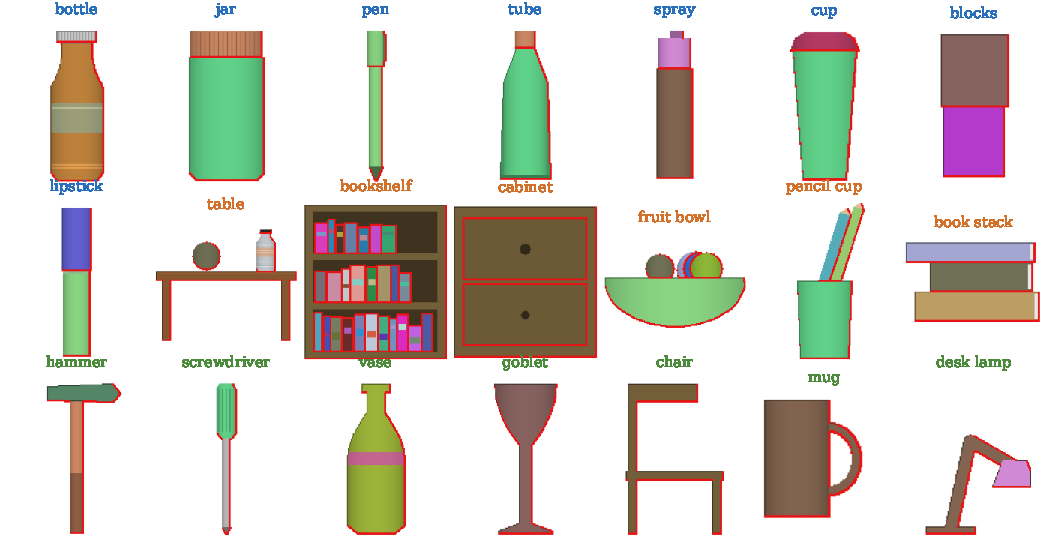
\includegraphics[width=\linewidth]{figures/scenes.pdf}
\caption{One test instance of each family with its ground-truth partition (red): single objects (blue titles), arrangements (orange), things that never come apart (green).}
\label{fig:scenes}
\end{figure}

\paragraph{Teaching.} A scripted hand handles each training scene: it carries the whole scene, then takes away up to three of its units one at a time (a unit is freed along its outline and dragged to free space; a cap only after its bottle has been taken off the table; a stack from the top down), then carries what is left; things that never come apart are carried twice. The hand never labels anything: the session observes the frames and the definition decides what came apart. Each scene is run once with an empty memory and its own state; the entries it produces are cached, and the memory for any training set is the union of its scenes' entries. We train on \nTrainPerFamily{} scenes per family (\nTrainScenes{} in all; \nEntries{} memory entries, \nPositives{} of them parts that came away) and test on \nTestPerFamily{} unseen still scenes per family (\nTestScenes{} in all).

\paragraph{Validation.} Four settings were chosen once, on \nValPerFamily{} further scenes per family with their own seeds, never used for testing: trait relevance on or off, $k\in\{3,4,6,8,12,24,48,96\}$, $\theta_+\in\{0.5,\dots,0.75\}$ and $w_0\in\{0.005,\dots,1\}$ (\nValConfigs{} combinations), each read exactly as the memory reads (checked numerically against it). The top of the validation surface is flat---many settings reproduce the same share of validation scenes to within one scene---so among the settings within one validation scene of the best exact-partition accuracy we took the one with the highest panoptic quality: relevance off, $k=\chosenK$, $\theta_+=\chosenTheta$, $w_0=\chosenW$ (validation accuracy \valAcc\%; the best setting with relevance on reached \valAccRel\%). This sequence matters for honesty: we first chose settings with relevance on, ran the test experiments, saw the unweighted variant do better on test, and only then added relevance to the validation grid; validation independently preferred it off, and all reported test results are from a fresh run with the validated settings. Test results use these values unless stated; the ablations vary them.

\paragraph{Ground truth and metrics.} The ground truth of a still scene is the finest partition its units induce, read at the patches; segments of fewer than three patches are void, as are patches that the image import placed in enclosed holes (inside a mug's handle), which sense paper. A prediction is the partition of \cref{sec:learning}. We report the share of scenes whose partition is reproduced exactly (every segment matched with IoU $>0.5$, nothing extra), panoptic quality PQ \citep{kirillov2019panoptic}, the recall of unit segments, false segments per scene, and---independently of the decision rule---the area under the ROC curve (AUROC) with which a scene's true units (candidates with IoU $\ge0.75$ to a unit) are ranked above its other candidates. Intervals are 95\% bootstrap intervals over test scenes, resampled within families. To make sure that evaluating from cached candidates is faithful, we ran the live session on \nEquivTotal{} test scenes with the full memory: its predicted partition agreed with the offline one on \nEquivAgree{} of them.

\paragraph{Baselines.} \emph{Never split}: the definition alone, before anything moves. \emph{Boundary contrast}: a part separates if its contact with the rest shows a strong signal change (edge median $+$ strong-edge share above a threshold fitted on the training entries for best F1)---classical segmentation by contrast. \emph{Logistic regression}: an L2-regularised, class-balanced linear classifier on the same standardised traits and the same weighted entries, decision at $0.5$. All methods use the same candidates, the same selection and the same partition step.

\section{Results}
\label{sec:results}

\paragraph{Main comparison.}
\Cref{tab:main} compares the memory with the baselines on all \nTestScenes{} test scenes. The definition alone (\emph{never split}) is right exactly on the \nWholeFam{} families that never come apart (\accNever\% of scenes). The memory reproduces the exact ground-truth partition of \accAll\% of scenes (95\% interval \accLo--\accHi\%), with PQ \pqAll\%: \accSingle\% of single objects, \accArranged\% of arrangements and \accWhole\% of things that never come apart. Logistic regression on the same traits and entries ranks true units about as well (its AUROC is higher) but its decision at $0.5$ splits almost everything: it finds more units and produces \fpLogistic{} false segments per scene against \fpLatent{} for the memory, and splits \splitWholeLogistic\% of things that never come apart against \splitWholeLatent\%. The boundary-contrast rule fares worse still (\accEdge\%): a strong edge is everywhere in these scenes---around a cap, but also around the painted band on a vase, a label on a book, the head of a hammer---and edges alone cannot tell which of them come apart. What separates the memory from both is not a better ranking but its abstention: a part is called separable only where enough stored parts that \emph{came away} sit nearby (\cref{prop:evidence}), and otherwise the definition's answer---one object---stands. Without the credible bound and support condition (\emph{no abstention}) accuracy falls to \accNoAbst\%.

\begin{table}[t]
\centering\small
\caption{Test scenes (\nTestPerFamily{} per family). Exact: share of scenes whose partition is reproduced exactly (95\% bootstrap interval); PQ: panoptic quality; unit recall: share of ground-truth units recovered; FP: false segments per scene; AUROC: ranking of true units among all candidates. All rows use the same candidates, selection and partition step.}
\label{tab:main}
\setlength{\tabcolsep}{4pt}
\begin{tabular}{@{}lrrrrrrrr@{}}
\toprule
 & \multicolumn{1}{c}{Exact (\%)} & PQ & single & arranged & whole & unit rec. & FP & AUROC \\
\midrule
\tabinput{tables/main.tex}
\bottomrule
\end{tabular}
\end{table}

\paragraph{Validated choices.} With the interactive application's original settings (relevance-weighted distance, $k=24$, $\theta_+=0.65$, $w_0=0.7$) the memory reaches \accDefault\%; the validated settings bring it to \accAll\%. Two of the changes are findings rather than tuning. First, weighting traits by their Fisher separation lowers accuracy (\accRelOn\% with the validated $k,\theta_+,w_0$). The weights it learns concentrate on the signal-edge traits (the largest: \relTop{}): parts that came away do have strong edges on average, so the criterion turns the distance into something close to an edge detector---and edges, as the boundary-contrast rule shows, are everywhere, including around parts that never come away. Equal weights keep the shape and contact traits in play, and those are what tell a cap from a painted band. Second, carried-whole entries are nearly worthless as evidence against separation (\cref{tab:ablation}): at their original weight $0.7$ accuracy on arrangements collapses to \arrCarriedSeven\%, because every carry of a bookshelf records book-shaped parts that stayed with it.

\paragraph{Candidate generators.} Straight cuts alone describe single objects well (\accCutsOnlySingle\% exact) but few of the arrangements (\arrCutsOnly\%); regions alone fail on single objects (\accRegionsOnlySingle\%, e.g.\ caps the colour of their body) and do better on arrangements (\arrRegionsOnly\%). Only their union does well on both.

\paragraph{Where it fails.} \Cref{fig:qualitative} shows predictions on test scenes. Over all separable families the memory recovers \unitsFound\% of the units. Arrangements are hard mostly because an exact partition needs \emph{every} unit: a test bookshelf holds up to \maxBooks{} books. Of the \arrMissed{} units missed in arrangements (out of \arrUnits), \missNotCalled\% had a candidate overlapping them well (IoU $\ge0.5$) that the memory did not call---it abstained for want of nearby parts that came away---\missNoCand\% had no such candidate at all (the generators did not propose the unit; \missNoCandShelf{} of these are books and \missNoCandCabinet{} drawers), and \missBadly\% were called but lost to an overlapping, worse-fitting candidate.

\begin{figure}[t]
\centering
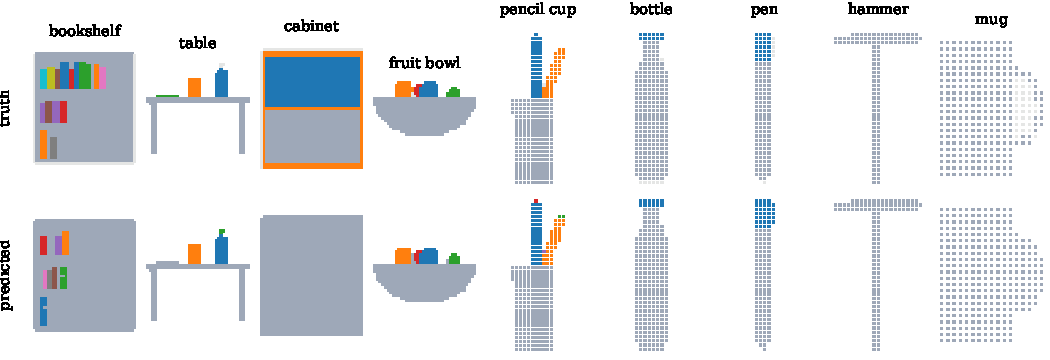
\includegraphics[width=\linewidth]{figures/qualitative.pdf}
\caption{Test scenes, nothing moved. Top: ground-truth partition (grey: void). Bottom: the memory's prediction (patches coloured by predicted object).}
\label{fig:qualitative}
\end{figure}

\paragraph{How much teaching.} \Cref{fig:curve} varies the number of handled scenes per family. Accuracy rises from \curveOne\% with one scene per family to \curveForty\% with \nTrainPerFamily{}, and has not levelled off. The gain is largest for single objects (\curveOneSingle\%$\to$\curveFortySingle\%), then arrangements (\curveOneArranged\%$\to$\curveFortyArranged\%). Things that never come apart start high (\curveOneWhole\%$\to$\curveFortyWhole\%): with nothing stored nearby that came away, the memory does not speak and the definition's answer stands; more teaching mainly removes the few false calls.

\begin{figure}[t]
\centering
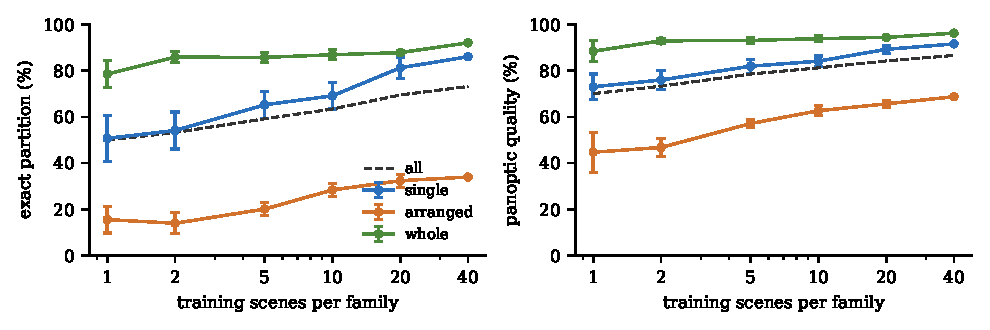
\includegraphics[width=\linewidth]{figures/curve.pdf}
\caption{Learning curves: exact-partition accuracy and PQ against the number of handled training scenes per family (mean $\pm$ s.d. over 5 random subsets).}
\label{fig:curve}
\end{figure}

\paragraph{New kinds of things.} \Cref{fig:lofo} removes each family from memory in turn and tests on it. Averaged over families, the memory reproduces \lofoMean\% of scenes of a family it has never seen (\lofoSingle\% for single objects, \lofoArranged\% for arrangements, \lofoWhole\% for things that never come apart), against \lofoMeanLogistic\% for logistic regression. Transfer between groups is weak: taught only single objects (and things that never come apart), it reproduces \trSA\% of arrangements; taught only arrangements, \trAS\% of single objects. Knowledge of what comes apart carries over between caps and lids of different single objects (a held-out single family is reproduced \lofoSingle\% of the time), but hardly between arrangements (\lofoArranged\%), and a book among books and a cap on a bottle are different enough in these traits that one does not teach the other. When a family is held out, the distance from its candidates to the nearest stored entry grows by a factor of \oodRatio{} (median), and the memory falls back on the definition.

\begin{figure}[t]
\centering
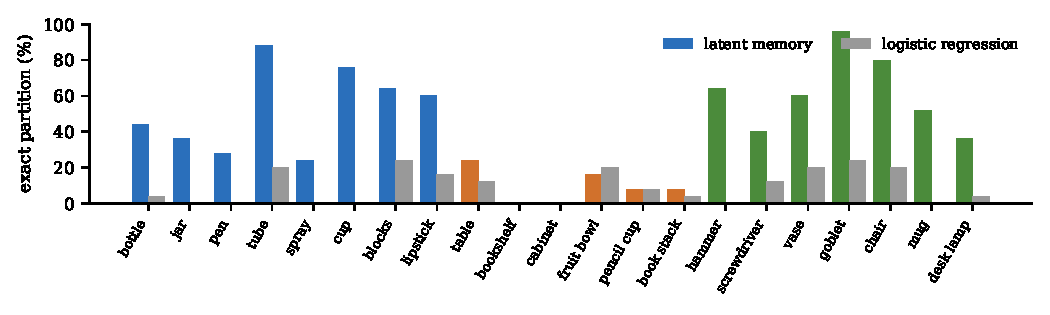
\includegraphics[width=\linewidth]{figures/lofo.pdf}
\caption{Leave-one-family-out: exact-partition accuracy on a family that is absent from memory (memory: all other families).}
\label{fig:lofo}
\end{figure}

\paragraph{Teaching a new kind.} \Cref{fig:fewshot} adds $k$ handled scenes of the held-out family to the memory of all others. Averaged over separable families, accuracy goes from \fsZero\% at $k=0$ to \fsTen\% at $k=10$ (single objects \fsZeroSingle\%$\to$\fsTenSingle\%, arrangements \fsZeroArranged\%$\to$\fsTenArranged\%). Consistent with \cref{prop:evidence}, one or two scenes change nothing on average (\fsOne\% and \fsTwo\%); five do (\fsFive\%). The memory states \emph{separates} only with three entries' worth of evidence nearby, and one handled scene contributes one to three. Families that never come apart gain too (right panel), although their carried-whole entries count almost nothing as evidence: what they change is \emph{who the neighbours are}. Once a few hammers are stored, a hammer's candidates find hammers among their $k=\chosenK$ nearest entries instead of distant parts that came away, and the memory stops calling separations it has no support for.

\begin{figure}[t]
\centering
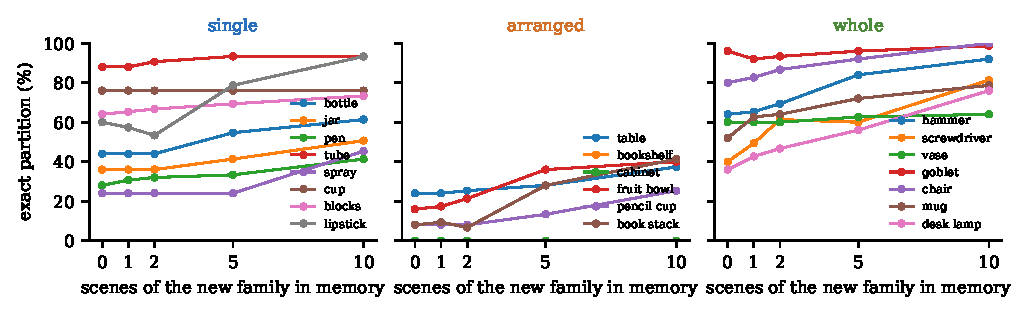
\includegraphics[width=\linewidth]{figures/few_shot.pdf}
\caption{Few-shot teaching of a family that was absent from memory: accuracy after adding $k$ handled scenes of it (mean over 3 random draws).}
\label{fig:fewshot}
\end{figure}

\paragraph{Ablations.} \Cref{tab:ablation} removes or isolates trait groups and varies the validated settings. \ablationText

\begin{table}[t]
\centering\small
\caption{Ablations on the test scenes (exact-partition accuracy and PQ, \%). Trait groups as in \cref{tab:traits}.}
\label{tab:ablation}
\begin{tabular}{@{}lrrrrr@{}}
\toprule
 & Exact & PQ & single & arranged & whole \\
\midrule
\tabinput{tables/ablation.tex}
\bottomrule
\end{tabular}
\end{table}

\paragraph{Robustness.} \Cref{tab:robust} applies changes never seen in training. A hue shift and dimmer light leave accuracy unchanged (\robRecolour\% and \robDark\%), as \cref{prop:invariance} predicts: only signal changes, normalised by the object's own, enter the traits. Turning pictures by $90^\circ$ costs some accuracy (\robRotNinety\%) and by $180^\circ$ much more (\robRotOneEighty\%): every trait but \emph{above} is invariant, and the drop shows how much the memory relies on parts resting on top of what they come away from. Shrinking to $0.7\times$ (\robScale\%) leaves fewer patches per part, near the resolution of the sensing. Sensor noise hurts most (\robNoise\%). Noise raises every neighbour difference, and with it the object's own typical difference that normalises the signal traits, so edges stand out less; it also fragments regions of similar signal. We have not separated these two effects. Under noise, logistic regression is as good as the memory (\robNoiseLogistic\%): a plausible reason, which we have not tested, is that noise makes candidates look unlike anything stored, so the memory abstains where a linear rule still extrapolates.

\begin{table}[t]
\centering\small
\caption{Robustness: test scenes changed in ways never seen in training (\nRobustPerFamily{} scenes per family).}
\label{tab:robust}
\begin{tabular}{@{}lrrrrrr@{}}
\toprule
 & \multicolumn{4}{c}{latent memory} & \multicolumn{2}{c}{logistic} \\
\cmidrule(lr){2-5}\cmidrule(lr){6-7}
change & Exact & PQ & arranged & whole & Exact & PQ \\
\midrule
\tabinput{tables/robust.tex}
\bottomrule
\end{tabular}
\end{table}

\paragraph{Calibration.} With the original settings, $\hat p$ is well calibrated as the probability that a candidate is a true unit (ECE \eceOriginal{}, \cref{fig:calibration}); with the validated settings it is not (ECE \eceChosen{}). The base rate is low---\baseRate\% of candidates are true units---and with carried-whole entries counting almost nothing, $\hat p$ in a neighbourhood without positives stays near the prior's $0.5$. Accuracy and calibration pull in different directions here: the validated memory decides well because it decides only with support, but its $\hat p$ should be read as the share of nearby \emph{weighted} evidence, not as a calibrated probability.

\begin{figure}[t]
\centering
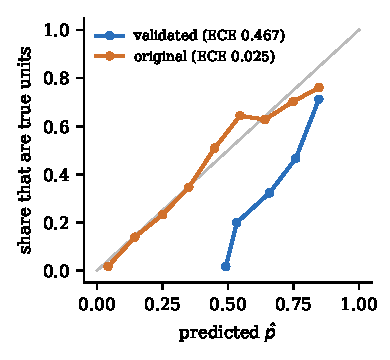
\includegraphics[width=0.45\linewidth]{figures/calibration.pdf}\hfill
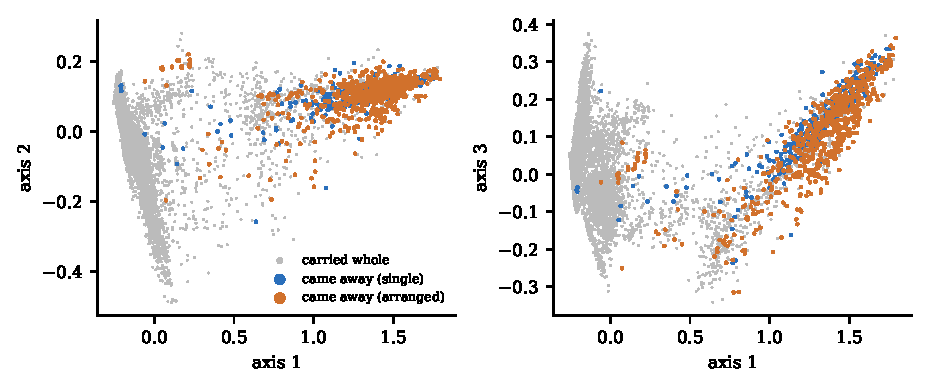
\includegraphics[width=0.53\linewidth]{figures/latent.pdf}
\caption{Left: reliability of $\hat p$ over all candidates of all test scenes (label: the candidate is a true unit, IoU $\ge0.75$). Right: the stored entries in the three directions of greatest spread of the standardised trait space; parts that came away (colour) occupy their own region, separate from parts that were carried whole (grey), for single objects and arrangements alike.}
\label{fig:calibration}
\end{figure}

\paragraph{Faithfulness of the evaluation.} The live session (the same code as the interactive application) with the full memory predicted exactly the partition the offline scoring computes on all \nEquivTotal{} test scenes we checked (\nEquivAgree{}/\nEquivTotal{}).


\section{Discussion and limitations}
\label{sec:discussion}

\paragraph{What the two layers buy.}
The definition alone is exact and never wrong about what has happened, but before anything moves it reports every scene as one object (\accNever\% exact partitions, almost all of them things that never come apart). The memory adds hypotheses about what would come apart, learned only from what the definition recorded, and \cref{prop:identity} guarantees that a wrong hypothesis can never corrupt identity: the moment a part is moved, the definition takes over. The memory is also inspectable: every reading can be traced to the stored entries that produced it (the application shows them live), and every entry to the event that created it.

\paragraph{Carried whole is weak evidence.}
The most consequential modelling choice turned out to be how much a \emph{carried-whole} entry counts. Carrying a bookshelf carries its books, yet books come out of shelves easily: being carried along says only that a part did not come away \emph{during that motion}. The definition's own wording is careful here---a patch set is one object because nothing has been \emph{observed} to open it---and the memory must be equally careful. Chosen on validation scenes, the weight of a carried-whole entry is $w_0=\chosenW$ against $1$ for a part that came away; the ablation shows how strongly arrangements depend on it. A principled alternative is to record which part the hand acted on: a part that was pulled and did not come away is strong evidence that it is attached, while a part that was merely carried with its support is almost none. Our session sees only patches, not the hand, so it cannot make that distinction yet.

\paragraph{Limitations.}
This is a study in a controlled world, and its conclusions are bounded by it.
(1) \emph{Sensing.} Patches lie on a lattice with known correspondence, position and visibility; real perception would have to track surfaces in depth and would add noise and occlusion. Thin diagonal structures break into fragments at our patch spacing, which the definition then correctly treats as separate objects (\cref{tab:teaching}); the definition's requirement that patches be fine enough to resolve every contact is a real constraint.
(2) \emph{Interaction.} The hand is scripted; it always takes away whole units and puts them in free space. Wide drawers dropped next to each other can hide one another, which accounts for most teaching outcomes that are not as intended.
(3) \emph{Traits and candidates.} The \nTraits{} traits are designed, physically motivated descriptors, not learned features; the memory learns only how much each counts. Candidates come from straight cuts and from regions of similar signal; a part that is neither---the same colour as its surroundings and bounded by a curved seam---cannot be proposed. The same-coloured pen caps are the clearest case of this.
(4) \emph{One behaviour.} Only coming apart is recorded. The memory's format allows others (opens, bends, rolls), each with its own relevance, but we have not studied them.
(5) \emph{Scale.} Reading is a linear scan over the memory, $O(N)$ per candidate; with \nEntries{} entries a test scene (about \candPerScene{} candidates) takes \secPerScene{}\,s on one machine. Larger memories would need approximate neighbour search. With $k$ fixed the estimate is not consistent (\cref{rem:consistency}).
(6) \emph{Comparisons.} Our baselines share the candidates, traits and decision structure, which isolates the reader; they do not include pixel-based segmentation models, which take a different input and supervision. A comparison on real images and real interaction is the obvious next step and would be the real test of whether physical traits of what came apart generalise beyond a procedural world.

\paragraph{Conclusion.}
An object can be defined by observation alone, and a system holding only that definition can still learn to anticipate what will come apart: by remembering the physical traits of what it saw separate and what it saw carried whole, and reading new things off their nearest remembered neighbours under a weighting the memory works out for itself. In a controlled world spanning caps and lids, books, drawers, fruit, pencils and things that never come apart, this recovers most unseen scenes exactly while leaving identity itself untouched.


\bibliographystyle{plainnat}
\bibliography{references}

\appendix
\section{Per-family results and teaching statistics}
\label{app:families}
\Cref{tab:families} gives per-family results and \cref{tab:teaching} what the scripted hand achieved when teaching.

\begin{table}[h]
\centering\small
\caption{Per family (test scenes). Exact and PQ: the memory with every family in memory; logistic: logistic regression, same setting; held out: exact accuracy when the family is absent from memory, and the share of its true units on which the memory then abstains; 5 shots: exact accuracy after adding five handled scenes of the family (mean of 3 draws).}
\label{tab:families}
\begin{tabular}{@{}lrrrrrr@{}}
\toprule
family & Exact & PQ & logistic & held out & abstains & 5 shots \\
\midrule
\tabinput{tables/families.tex}
\bottomrule
\end{tabular}
\end{table}

\begin{table}[h]
\centering\small
\caption{Teaching (\nTrainPerFamily{} scenes per family). Units taken: units the hand took away per scene. As intended: share of scenes in which the definition ended with one object more per unit taken, ignoring fragments under five patches (and counting them: strict). Positives and carried: memory entries recorded.}
\label{tab:teaching}
\begin{tabular}{@{}llrrrrr@{}}
\toprule
family & group & units taken & as intended & strict & positives & carried \\
\midrule
\tabinput{tables/teaching.tex}
\bottomrule
\end{tabular}
\end{table}


\end{document}
